\chapter{Enforcement of \eapABAC{} Models}
\label{sec:enforcements}
In this chapter, we demonstrate usefulness of EAP models by demonstrating enforcement in application contexts. We particularly use \eapABAC{} to design a protection model for JSON documents. We have implemented this protection model in OpenStack Swift storage.  The implementation allows ``policy-based selective access'' of stored OpenStack Swift objects instead of Swift's default ``all/no access''. In the following sections of this chapter, we briefly discuss motivations for this work, required background of JSON documents, enforcement models, security-policy syntax and finally implementation and its evaluation. 

%\section{Protection Model for JSON Documents}
%	In this section, we design a protection model for JSON documents. In the following sub-section, we discuss our motivation for choosing JSON data model. We also discuss salient properties of semi-structured JSON data, and justify our approach over existing XML protection mechanisms. 
	
	\subsection{Motivation}
JavaScript Object Notation (JSON) is a human and machine readable representation for text data.  It is widely used because of its simple and concise structure.  For example, Twitter uses  JSON as the only supported format for exchange of data starting from API v1.1 \cite{twitter-api} and YouTube  recommends uses of JSON for speed from its latest API \cite{youtube-api}.  JSON  is being adapted increasingly in  large and scalable document databases such as MongoDB \cite{mongodb}, Apache Casandra \cite{cassandra} and CouchDB \cite{couchdb}. Besides  these, JSON is also widely used in lightweight data storages for example in configuration files, online catalogs or  applications with embedded-storage.


%For the high adoption of these document databases,  recently, OpenStack  Database service, Trove, provides support for MongoDB starting from  Icehouse release \cite{openstack-support-mongodb}

In spite of high adoption from industries, JSON has received little attention from academic researchers. To the best of our knowledge, there is no formal work published  on the protection of JSON documents.


On the other hand, considerable work has been done for protection of XML documents. Although syntactically JSON and XML formats are different, semantically both of them form a rooted tree hierarchical structure. In fact, JSON data can equivalently be represented in XML form and vice versa. This brings an obvious question -  whether we can utilize  authorization models used for XML documents for protection of  JSON data.


% 
 	\begin{figure} 
 		\centering
 		\includegraphics[width=.9\textwidth]{example-json-data}
 		\caption{Example of JSON Data}
 		\label{fig:example-json-data}
 	\end{figure}
 

Before we answer the preceding question, we look into some of the salient characteristics of data represented in JSON (or XML) format, given below.  

%In Figure \ref{fig:example-json-data} (a) we present employee records in a flat JSON file. The same records has been re-organized and presented in Figure \ref{fig:example-json-data} (b).  We believe, the key characteristics of JSON data to be considered for specification of authorization policies are as follows.

\begin{itemize}
	
	\item \textbf{Hierarchical relationship.} Data often exhibits hierarchical relationship. For example, a residential address consists of pieces like house number, street name, district/town and state name organized into an strictly hierarchical structure. 
	
	
	\item \textbf{Semantical association.} Different pieces of data are often related semantically and may need same level of protection.  For example, phone number, email address, Skype name may all represent contact information and require same level of protection.
	
	\item \textbf{Scatteredness.} Related information can be scattered around a document. For example, different pieces of contact information might be located in different places in a document. Some pieces of data can even be repeated in more than one place in the same document or across documents.  
	
	%For example, \ref{fig:example-json-data} (b), \textit{email} and \textit{work-phone} is placed under both \textit{public-info} and \textit{contact-info}.
\end{itemize}




Interestingly, most of XML authorization models \cite{policy-based4,policy-based2,policy-based5,policy-based6} consider \textit{structural hierarchy} only. These models have an implicit assumption that information has been organized in the intended hierarchical form. These models attach authorization policies directly on nodes in the XML tree  and propagate them using the hierarchical structure. For example, Damiani et al. \cite{damiani2002fine} specify authorization policy as a tuple $\langle subject, object, action,$ \\ $sign, type \rangle$ where subject is specified as user, user group, IP address or semantic name;  object is specified with XPath expression; example of actions are read or  write; signs are positive and negative; and example of types are local, global and DTD which determines the level of propagation.  In this model, if similar data items requiring same level of protection are placed in structurally unrelated nodes, it is required to attach same authorization policy to all these nodes. This results in duplication of authorization policies which is caused by lack of recognition of semantical association and scatteredness properties. 

%Propagation of authorization policies in these model is solely based on structural hierarchy. As a result, these models suffer in the maintenance of authorization policies. 

Duplication incurs significant overhead in maintenance of authorization policies. For instance, if requirements for storing or publishing contact information (e.g. email, phone, fax) change, it is required to update policies for all different pieces of data that represent contact information. Organizations often collect different types of data including personal identifiable information of employees and customers. So, they are compliant to different internal and external parties including government and standard bodies. This increases the likelihood that authorization requirements change frequently over time. 

% This also increases the possibility of  inconsistencies due to unintended mistakes. 


%\textbf{Duplicated authorization policies.} If an XML element appear in more than one nodes (for example, in Figure \ref{fig:example-json-data} \textit{email} appears in two different node), we need to duplicate the same authorization policies in each node. While we need to update authorization policies, we need to update all duplicated policies. Assuming policy update is not infrequent, this poses significant maintenance overhead. 

While most XML authorization models directly identify nodes in their authorization policies, our proposed model adds a level of abstraction by using \textit{security-label} attribute values. The proposed model specifies two types of policies called \textit{authorization policies} and \textit{labeling policies}.  Authorization policies are specified using \textit{security-label} attribute values. These values are assigned to JSON data using labeling policies. A conceptual overview of existing XML authorization models and our proposed model is  shown schematically in Figure \ref{fig:indirection}(a) and \ref{fig:indirection}(b) respectively. By using security-label attribute values to connect nodes and policies, we can assign semantically related or scattered data same attribute values. This eliminates the need to specify duplicated policies.
	
 
 	\begin{figure} [t]
 		\centering
 		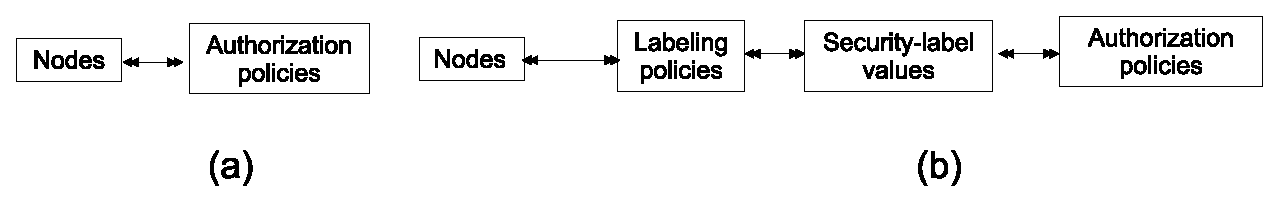
\includegraphics[width=.9\textwidth]{NSS16/indirection}
 		\caption{(a) Existing XML models  (b) the proposed model}
 		\label{fig:indirection}
 	\end{figure}
 
	
%In this paper, we propose attribute based specification of authorization policies for protecting JSON document. Though we consider JSON data, the same protection model can also be used for XML documents as well. We consider one user attribute called \textit{user-label} or  \textit{uLabel} in short and one object attribute called \textit{security-label} or \textit{sLabel} in short. \textit{uLabel} values are assigned on users and \textit{sLabel} values are assigned on JSON elements. For each authorization action, we specify one policy consisting of enumerated micro-policies using these labels.  For example, the authorization policy $Auth_{read}$= \textit{\{(HR, contact-info)\}} specify that all users who are assigned value \textit{HR} can read all JSON objects which are assigned value \textit{contact-info}. Our protection model is adapted from the enumerated ABAC model\cite{labac}. 






The proposed model additionally offers flexibility in specification and maintenance of  authorization and labeling policies. These two types of policies can now be managed separately and independently. For instance, given \textit{security-label} attribute values, higher level, organization-wide policy makers can specify authorization policies using these values without knowing details of JSON structure. On the other hand, local administrators knowledgeable about details of specific JSON documents can specify labeling policies. 


We believe, the presented model can easily be generalized for data represented in trees and be instantiated for other representations, for example, YAML \cite{yaml}. For simplicity, we only focus on JSON here.


\section{The Operational Model}


 
 	\begin{figure}[t]
 		\centering
 		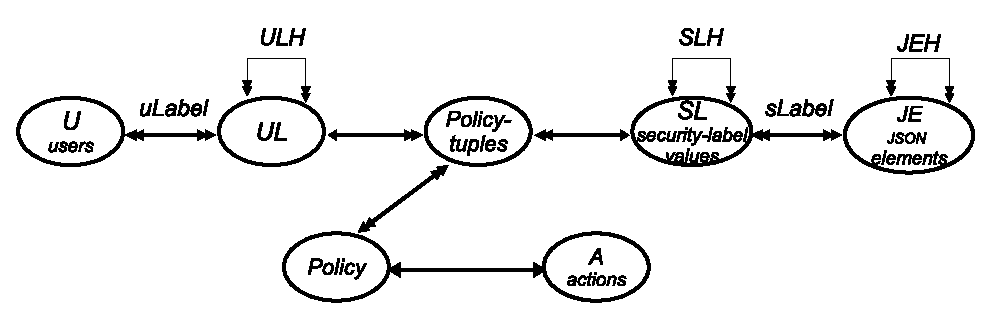
\includegraphics[width=.9\textwidth]{NSS16/operational-model}
 		\caption{ The Attribute-based Operational Model (\atom{})}
 		\label{fig:operational-model}
 	\end{figure}
 


\label{sec:operational-model}


This section presents the Attribute-based Operational Model (\atom{}) for protection of JSON documents. \atom{} adapts enumerated authorization policies from  \cite{labac,eap-abac}.


\begin{table}[t]
	\centering
	\caption{ Definition of \atom{}} %\vspace*{3pt}
	\label{tab:operational-model}			
	\begin{tabular}{|l|}

		\hline					
				\begin{tabular}{l}
							\multicolumn{1}{c}{\underline{\textit{I. Sets and relations }}}\\			
							- \textit{U, JE} and $A$  (set of users, JSON elements and actions respectively)  \\
							- \textit{JEH} (hierarchy of JSON elements, represented by $\JEH$) \\
							- \textit{UL} and \textit{ULH} (finite set of uLabel values and their partial order denoted as $\udominate$ respectively) \\
							- \textit{SL} and  \textit{SLH} (finite set of security-label values and their partial order denoted as $\odominate$ respectively) \\
							- $\uLabel$ and $sLabel$ (attribute functions on users and JSON objects respectively) \\
							 \hfil Formally, $\uLabel: U \to 2^{UL}$; $\oLabel: JO \to 2^{SL}$ \\														

							 \multicolumn{1}{c}{\underline{\textit{II. Policy components}}} \\	
							 - $\policyTuples{} = UL \times SL$\\			
							- $Policy_a \subseteq \policyTuples{}$ for $a \in A$ \\
							-  $Policy = \{Policy_a | a \in A\}$ \\
							\multicolumn{1}{c}{\underline{\textit{III. Authorization function}}} \\						
							%- $\request(u:U, a:A, je_i:JE)$ =	($\forall je_j \preceq je_i$ ($\exists ul_i \in \uLabel(u), \exists sl_m \in \oLabel(je_j),$ \\ \hfill$\exists (ul_j, sl_n) \in Policy_a $) ) $[ul_i \udominate ul_j \land sl_m \odominate sl_n]$ 
							- $\canAccess (u:U, a:A, o:JE) =  (\exists (ul,sl) \in Policy_a) [ul \in \uLabel(u) \land sl \in \oLabel(o)]$\\
							- $\request(u:U, a:A, je_i: JE) \equiv \exists je_j [(\canAccess(u,a,je_j)) \land je_i \odominate je_j]$ \\
							
				\end{tabular}
					
			
 \\ \hline	
	\end{tabular}
	
\end{table}



  	\begin{figure} [t]
 		\centering
 		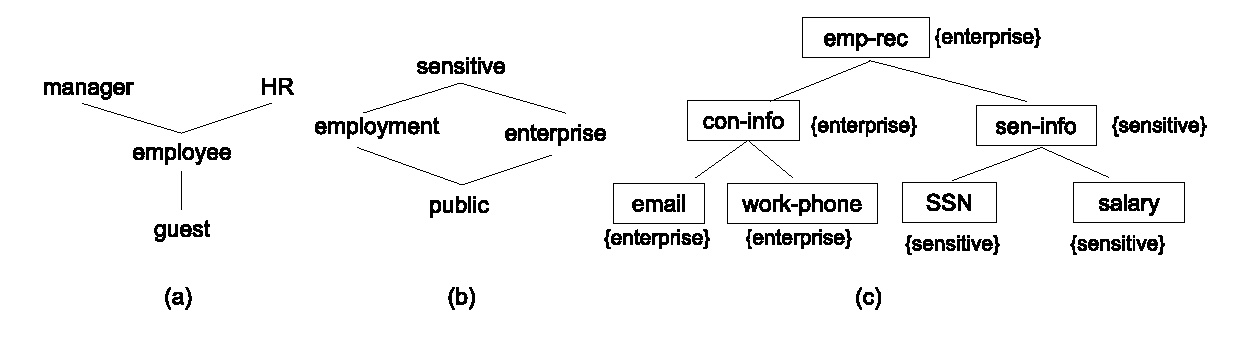
\includegraphics[width=1\textwidth]{NSS16/operational-explanation}
 		\caption{(a) User-label values, (b) Security-label values and (c)  Annotated JSON tree}
 		\label{fig:operational-explanation}
 	\end{figure}
 
\begin{table}[t]
\centering
\caption{Example of an authorization policy and authorization requests}
\label{tab:example-auth-policy}
\begin{tabular}{|l|}
	\hline
%\textit{}                      \\ \hline
\multicolumn{1}{|c|}{\textit{\underline{I. Enumerated authorization policies}}} \\   
$Policy_{read} \equiv$ \{ \textit{(manager,sensitive), (HR,employment)}, \\ \hfill \textit{(employee, enterprise), (guest, public)}\}\\ \hline

\multicolumn{1}{|c|}{\textit{\underline{II. Authorization requests}}} \\   
$\request(Alice,read, \textit{emp-rec}) = true$, assuming $\uLabel(Alice)=\{manager\}$\\
$\request(Bob,read, \textit{emp-rec}) = false$, assuming $\uLabel(Bob)=\{employee\}$\\
$\request(Bob,read, \textit{con-info}) = true$, assuming $\uLabel(Bob)=\{employee\}$\\
$\request(Charlie,read, \textit{sen-info}) = false$, assuming $\uLabel(Charlie)=\{HR\}$\\
\hline
\end{tabular}
\end{table}


%$ Policy_{read} \equiv \{(Visitors, public\_data), (HR, persona\_data),(HR, employment\_data),$  \\\hfil $(employee, protected\_data),(manager,sensitive\_data)\}$         \\ \hline
%$Policy_{write} \equiv \{(HR, personal\_data),(HR, employment\_data),$ \\ \hfil $(director, sensitive\_data)\}$ \\ \hline

Figure \ref{fig:operational-model} presents components of \atom{}. In the figure, the set of users is represented by $U$. Each user is assigned to one or more values of an attribute named \textit{user-label} or \textit{uLabel} in short. These values are selected from the set of all possible user-label values $UL$ which are partially ordered. The partial order is represented by $ULH$. An example showing user-label values and  hierarchy is presented in Figure \ref{fig:operational-explanation}(a). On the other hand, the set of JSON elements are specified as \textit{JE}. JSON elements may subsume other JSON elements, and form a tree structured hierarchy. The hierarchy is represented by \textit{JEH}. Each JSON element is assigned values of an attribute named \textit{security-label} or \textit{sLabel} in short. These values are selected from the set of security-label values $SL$ which are also partially ordered. The partial order is represented by \textit{SLH}. An example showing security-label values and  hierarchy is presented in Figure \ref{fig:operational-explanation}(b). A JSON tree annotated with security-label values is given in Figure \ref{fig:operational-explanation}(c). These components and relationship among them are formally specified in Segment I of Table  \ref{tab:operational-model}.

% The many-to-many relation between JSON elements and security-label values are specified by the attribute function \textit{sLabel}In an organization, it is possible to have an existing classification system that categorizes all objects or resources in the organization. Such a classification system can be used to derive security-label values and its hierarchy. 

In Figure \ref{fig:operational-model}, the set of authorization policies is represented by \textit{Policy}. There exists one authorization policy per action which is shown by the one-to-one relation between  \textit{Policy} and the action \textit{A}. In Table \ref{tab:operational-model}, $Policy_{read}$ presents the authorization policy for  action read. An authorization policy may contain one or more micro-policies, and one micro-policy can be associated with more than one authorization policy. This is represented by the many-to-many relation between \textit{Policy} and \textit{Policy-tuples}. $Policy_{read}$, as mentioned above, contains four policy-tuples including \textit{(manager, sensitive)}. The tuple \textit{(manager, sensitive)} in policy $Policy_{read}$ specifies that users who are manager can read objects that have been assigned values sensitive. Formally, we represent a policy-tuple as a pair of atomic values $(ul, sl)$ where $ul \in UL$ and $sl \in SL$. The formal definition of policies and policy-tuples is given in Segment II of Table \ref{tab:operational-model}. We use the terms policy-tuples and micro-policies equivalently to represent sub-policies.

%The formal definition of \atom{} is given in Table \ref{tab:operational-model}. In Section I of the table, we formally specify the sets and relations used in the model as described above. Section II formally specifies the relationship among policies, actions and policy-tuples. 

The authorization function $\request{}()$ is specified in Section III of Table \ref{tab:operational-model}. We define the helper function $\canAccess{}(u,a,o)$ which specifies that the user $u$ can access the object $o$ for action $a$ if there exists a policy-tuple in $Policy_{a}$ that allows it. A user is authorized to perform an action on the requested JSON element  if he can access the requested element and all its sub-elements. For example, let us assume, Alice as a manager wants to read \textit{emp-rec} which has been assigned value \textit{enterprise} as shown in Figure \ref{fig:operational-explanation}(c). The tuple \textit{(manager, sensitive)} in $Policy_{read}$ specifies that Alice can read object labeled with sensitive or junior values. Thus, the request $\request$\textit{(Alice, read, emp\_rec)} is evaluated as true. On the other hand, assuming Bob as an employee, the request \textit{\request(Bob, read, emp-rec)} is evaluated as false as an employee cannot read \textit{sen-info} which is sub-element of \textit{emp-rec}. Additional examples of authorization request are given in Segment II of Table  \ref{tab:example-auth-policy}.




\newcommand{\assignmentControl}{\textit{assignment-control}}
\newcommand{\propagationControl}{\textit{propagation-control}}
\section{Labeling Policies}
\label{sec:administrative-model}
 


 
 In this section, we discuss specification of labeling policies for the operational model given in Section \ref{sec:operational-model}. We broadly categorize the policies used in the operational model into specification of authorization policies and assignment of security-label values or labeling policies. Policy scope of the operational model is schematically shown in Figure \ref{fig:administration-scope}. Here, we focus on the later type of policies.
 
   
 	\begin{figure} [t]
 		\centering
 		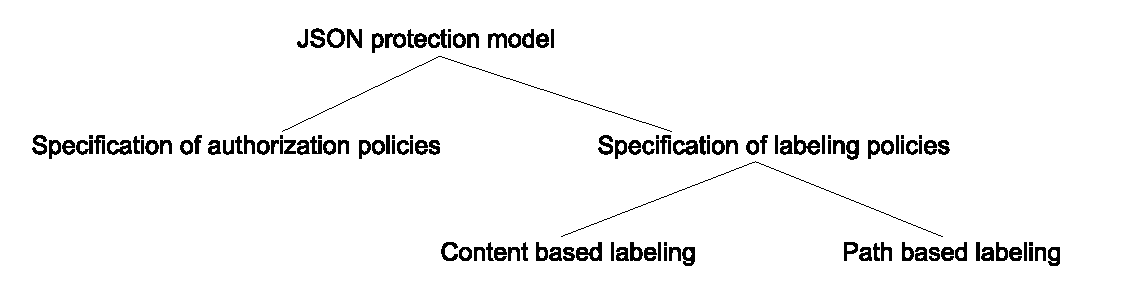
\includegraphics[width=1\textwidth]{NSS16/administration-scope}
 		\caption{Policy scope}
 		\label{fig:administration-scope}
 	\end{figure}
 
 
 We specify two different approaches to assign security-label values to elements in a JSON document, viz. content-based and  path-based. These approaches are fundamentally different in how a JSON element is specified. While a path is described starting from the root node of the tree, content is specified starting from the leaf nodes of the tree. These two contrasting approaches offer flexibility in assignments and propagation of security-label values.
 
 %The scope of administration is shown in Figure \ref{fig:administration-scope}. We broadly categorize administrative scope into administration of authorization policies and assignment of security-label values. The former is related to administration of enumerated authorization policy ABAC models which is an interesting problem of its own. This paper only discusses assignments of security-label values in the context of JSON documents.
 
 \subsection{Control on Labeling Policies}
 
 

For specification of labeling policies, we define two types of restriction that control assignments and propagations of \textit{security-label} values. In the first type, we restrict how security-label values are selected and assigned on tree nodes. We call this \assignmentControl{}. In the second type, we specify how assigned values are propagated along nodes in the tree. We call this \propagationControl{}. 
 
  	\begin{figure} [t]
 		\centering
 		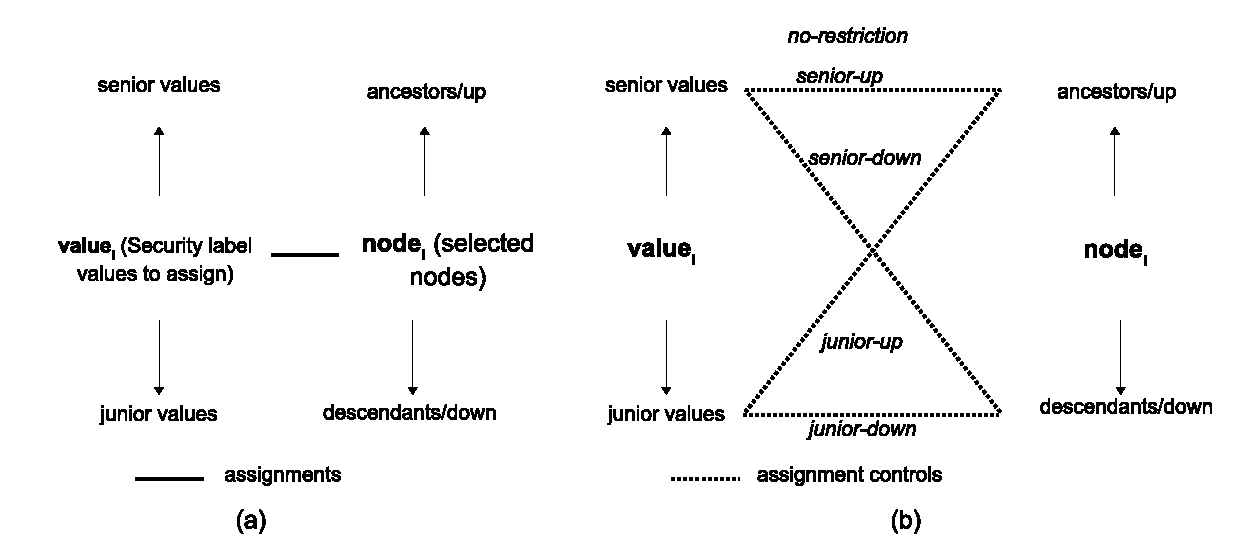
\includegraphics[width=1\textwidth]{NSS16/assignment-control}
 		\caption{Demonstration of (a) assignment of security label values and (b) assignment controls}
 		\label{fig:restriction-types}
 	\end{figure}
 
 
 The motivation of \assignmentControl{} is to restrict arbitrary assignments of security-label values. This enables administrators to restrict future assignments after some assignments have been carried out.  These controls are specified during the assignments. If any attempting assignment does not comply with \assignmentControl{}s of existing assignments, it will be rejected. We define five possible options for \assignmentControl{} as \textit{no-restiction}, \textit{senior-up}, \textit{senior-down}, \textit{junior-up} and \textit{junior-down}. The type \textit{no-restriction} does not specify any restriction. If we assign a value $value_i$ in $node_i$, with \textit{senior-up} restriction, all up/ancestors of $node_i$ must be assigned values senior to $value_i$ possibly including $value_i$. In type \textit{senior-down} restriction, all down/descendants of $node_i$ must be assigned values senior to $value_i$ possibly including $value_i$.  Similarly, the types \textit{junior-up} and \textit{junior-down}, specify that ancestors and descendants of $node_i$ must be assigned  values junior to $value_i$, possibly including $value_i$.  Figure \ref{fig:restriction-types} schematically illustrates \assignmentControl{}. In Figure \ref{fig:propagation-option}, the node \textit{con-info} is assigned a value \textit{enterprise} with option \textit{junior-down} which regulates that its descendant nodes namely \{email, work-phone\} must be assigned values $enterprise$ or its juniors, in this case from the set \{enterprise, public\} (using security-label values given in Figure \ref{fig:operational-explanation}(b)). In the same figure, the node \textit{sen-info} is assigned value \textit{sensitive} with option \textit{senior-down} which mandates that its descendant nodes namely \{SSN, salary\} must be assigned values from \textit{sensitive} or its seniors, in this case from the set \{sensitive\}.

%We define \textit{labeling options} to control how  security-label values are assigned to JSON elements. Possible options are \textit{unrestricted}, \textit{restricted-up} and \textit{restricted-down}. If unrestricted, a node can be assigned any security-label values allowed in the system. We can impose restriction for the assignments by using the options \textit{restricted-up} and/or \textit{restricted-down}. When we assign a value $V_i$  on a node $N_i$ (which is not unrestricted by existing assignments) with the option \textit{restricted-up}, it requires that all ancestor nodes (of $N_i$) must be assigned values equal or senior to $V_i$. Similarly, the option \textit{restricted-down} requires that all descendant nodes must be assigned a value equal or junior to $V_i$. Using these options, we can restrict the possible values that can be assigned to a node. Figure \ref{fig:propagation-option} explains how these options pose restriction for assignments of  security-label values on nodes in the tree. For example, 

   
 	\begin{figure} [t]
 		\centering
 		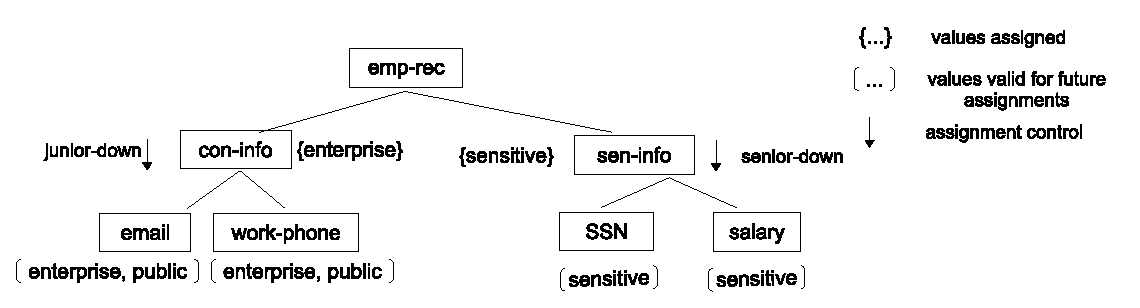
\includegraphics[width=1\textwidth]{NSS16/propagation-option}
 		\caption{Assignments with assignment controls}
 		\label{fig:propagation-option}
 	\end{figure}
% (considering security-label value hierarhcy given in Figure \ref{fig:operational-explanation})


 Once we assign security-label values on an element in a JSON tree, the value can be propagated to other elements in the tree. We define following  types for \propagationControl{} as \textit{no-prop},  \textit{one-level up}, \textit{one-level down},  \textit{cascading up} and \textit{cascading down}. Assigned values are not propagated in type \textit{no-prop}. From a node, assigned values are propagated to parent and all its siblings in the type \textit{one-level up}. Assigned values are propagated to all ancestor nodes in type \textit{cascading up}. Similarly, from a selected item, assigned values are propagated to direct children in type \textit{one-level down} and to all descendants in type \textit{cascading down}. % Propagation types are explained with an example in Figure \ref{fig:propagation-types}. 
 
%  
 	\begin{figure} [t]
 		\centering
 		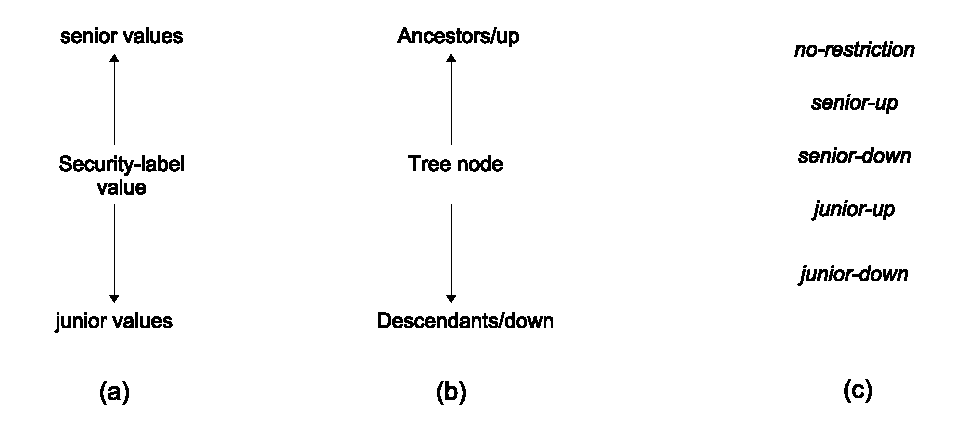
\includegraphics[width=1\textwidth]{propagation-types}
 		\caption{Example explaining propagation types}
 		\label{fig:propagation-types}
 	\end{figure}
 
 

\subsection{Content-based Labeling}

  
 	\begin{figure} [t]
 		\centering
 		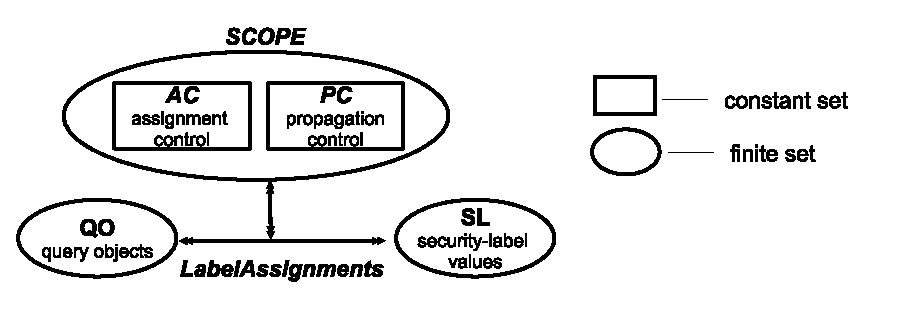
\includegraphics[width=1\textwidth]{NSS16/QO-based-labeling}
 		\caption{Content-based labeling model}
 		\label{fig:QO-based-labeling}
 	\end{figure}
  
\begin{table}[t]
	\centering
	\caption{Definition of content-based labeling} %\vspace*{3pt}
	\label{tab:QO-labeling-definition}			
	\begin{tabular}{|l|}
		\hline					
		\begin{tabular}{l}
			
				\multicolumn{1}{c}{\underline{\textit{I. Basic sets and relations}}}\\													
					
					- $QO$ (set of query objects). \\
					- $AC$ (assignment control) $AC$= \textit{\{no-restriction, senior-up, junior-up\}}.\\
					- $PC$ (propagation control) $PC = \{\noProp, \oneLevelUP, \cascadeUP\}$.\\

					- $SCOPE \subseteq  AC \times PC$\\
					- $SL$ (set of security-label values). \\
									
					\multicolumn{1}{c}{\underline{\textit{II. Assignments of security-label values}}}\\					
					- $\labelAssignment \subseteq QO \times SCOPE \times 2^{SL}$ \\ 

		\end{tabular}			
		 \\ \hline	
	\end{tabular}
	
\end{table}




This section shows how to assign security-label values by matching content and propagating the labels.

We adapt the concept of \textit{query object} available in MongoDB \cite{mongodb} which matches content in a JSON document. Query objects discover content starting from the \textit{value nodes} of the JSON tree. A query object accepts regular expression to find \textit{value nodes}  or \textit{key nodes} conveniently. MongoDB has built-in functions to express regular expressions and compare values matched by the regular expressions. 

A model to assign {security-label} values based on query objects is given in Figure \ref{fig:QO-based-labeling}. In the figure, $QO$ represents the set of all query objects and $SL$ is the set of {security-label} values. The set $AC$ represents \assignmentControl{} and $PC$ represents \propagationControl{} discussed earlier.  $AC$ and $PC$ together define labeling scopes. A labeling scope determines how values are assigned and propagated in the tree. As content is matched from the value/leaf nodes of the tree, we consider assignment and propagation control only for the ancestors of the matching nodes.

The formal definition of the model is given in Table \ref{tab:QO-labeling-definition}. Segment I of the table specifies basic sets and relations. In Segment II, the relation \textit{ \labelAssignment{}} defines rules for assigning security-label values. An assignment rule is a triple of a query object to match content, a scope and a set of values to be assigned.  Section I of  Table \ref{tab:content-based-example} gives some examples of query objects and their interpretation in plain English.  Segment II of Table \ref{tab:content-based-example}, presents examples of assignment policies based on query objects.


\begin{table}[t]
	\centering
	\caption{ Examples of query objects and content-based labeling policies} %\vspace*{3pt}
	\label{tab:content-based-example}			
	\begin{tabular}{|l|}
		\hline					
		\begin{tabular}{l}
				\multicolumn{1}{c}{\underline{\textit{I. Query objects}}}\\										
				- ob1 = \{``email": \{ \$regex:``/.*@example.com/"\} \} (matches email addresses \\ \hfil from domain example.com)  \\
				- ob2 = \{ \$elemMatch: \{ \$regex: ``\reForEmail''  \} \} (matches any key having value \\ \hfil  corresponding to the  given regular expression) \\  
				- ob3 = \{\$elemMatch:\{ \$regex: ``\reSSN"\}, \$elemMatch: \{``\reCreditCard"\}\} \\ \hfil (matches all objects containing both social security and credit card number) \\
					
				\multicolumn{1}{c}{\underline{\textit{II. \labelAssignment}}}\\			
				- \labelAssignment = \{ (ob1, (no-prop, unrestricted), \{enterprise\}),   (ob2,\\ \hfil (no-prop, unrestricted),  \{enterprise\}), (ob3, (no-prop, restricted), \{ sensitive\} \}				\\
		\end{tabular}			
		 \\ \hline	
	\end{tabular}
	
\end{table}



 
 	\begin{figure}[t]
 		\centering
 		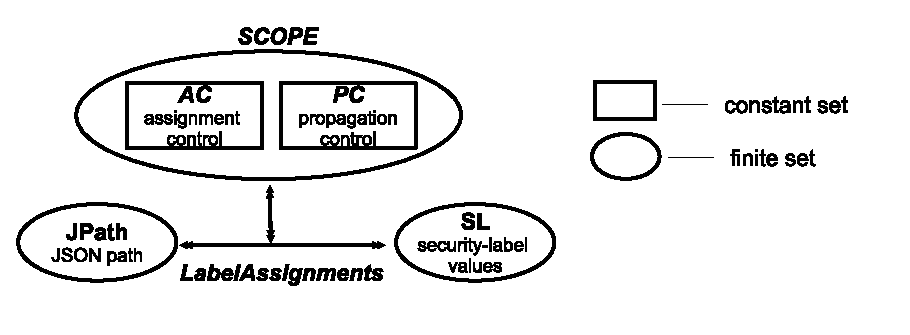
\includegraphics[width=1\textwidth]{NSS16/path-labeling-model}
 		\caption{Path-based labeling model}
 		\label{fig:path-based-labeling}
 	\end{figure}
 
\begin{table}[t]
	\centering
	\caption{Definition of Path-based labeling} %\vspace*{3pt}
	\label{tab:Path-labeling-definition}			
	\begin{tabular}{|l|}
		\hline					
		\begin{tabular}{l}
			
				\multicolumn{1}{c}{\underline{\textit{I. Basic sets and relations}}}\\	
					- $JPath$ (set of JSONPaths). \\
					- $AC$ (assignment control) $AC$= \textit{\{no-restriction, senior-down, junior-down\}}.\\
					- $PC$ (propagation control) $PC = \{\noProp, \oneLevelUP, \cascadeUP\}$.\\
					
					- $SCOPE \subseteq  AC \times PC$, relation to assign and propagate values.\\
					- $SL$ (set of security-label values). \\
									
					\multicolumn{1}{c}{\underline{\textit{II. Assignments of security-label values}}}\\					
					- $\labelAssignment \subseteq JPath \times SCOPE \times 2^{SL}$ (assign security-label values on \\ \hfill JSON elements matched and  propagate  values based on defined scope) \\ 

		\end{tabular}			
		 \\ \hline	
	\end{tabular}
	
\end{table}




\subsection{Path-based Labeling}

In this section, we show how we assign security-label values by matching paths in the JSON tree and propagating them along the tree. 

We adapt \textit{JSONPath} \cite{JSONPath} to specify path-based labeling policies. This model is very similar to the content-based labeling model except we use JSONPath instead of query objects. While, query objects are matched starting from the leaf nodes, JSONPath specifies elements starting from the root node (or any node in case of relative path) and traverses towards a leaf of the tree. As a result, this model apply assignment control and propagation control towards descendants of matching nodes.  The components of the model and its formal definition are given in Figure \ref{fig:path-based-labeling} and Table \ref{tab:Path-labeling-definition} respectively. Examples of JSON paths and path based labeling policies are presented in Segment I and II of Table \ref{tab:path-based-example}.


\begin{table}[t]
	\centering
	\caption{ Examples of JSONPath and path-based labeling policies} %\vspace*{3pt}
	\label{tab:path-based-example}			
	\begin{tabular}{|l|}
		\hline					
		\begin{tabular}{l}
				\multicolumn{1}{c}{\underline{\textit{I. JSONPaths}}}\\										
				- {path-to-email}=\$.{emp-rec.con-info.email}\\					
				- {path-to-salary}=\$.{emp-rec.sen-info.salary}\\
				\multicolumn{1}{c}{\underline{\textit{II. \labelAssignment}}}\\			
				- \labelAssignment = \{ (path-to-email, (no-prop, unrestricted), \{enterprise\}),  \\ \hfil (path-to-salary, (no-prop, unrestricted),  \{sensitive\}) \}				\\
		\end{tabular}			
		 \\ \hline	
	\end{tabular}
	
\end{table}



 % administrative model




\subsection { Implementation in OpenStack Swift}
\label{sec:implementation}

 \begin{figure} [t]
 	\centering
 	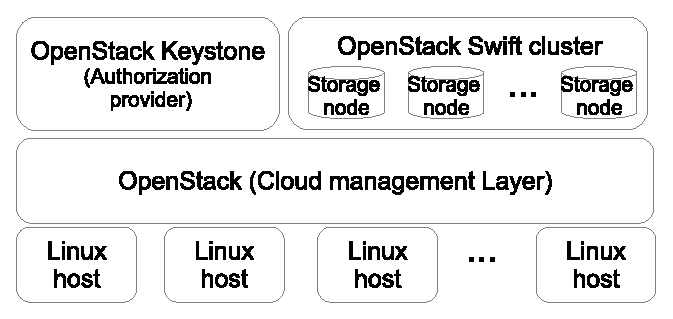
\includegraphics[width=.6\textwidth]{NSS16/reference-implementation-architecture}
 	\caption{Reference architecture of the implementation testbed}
 	\label{fig:reference-implementation-architecture}
 \end{figure}


 
 	\begin{figure} [t]
 		\centering
 		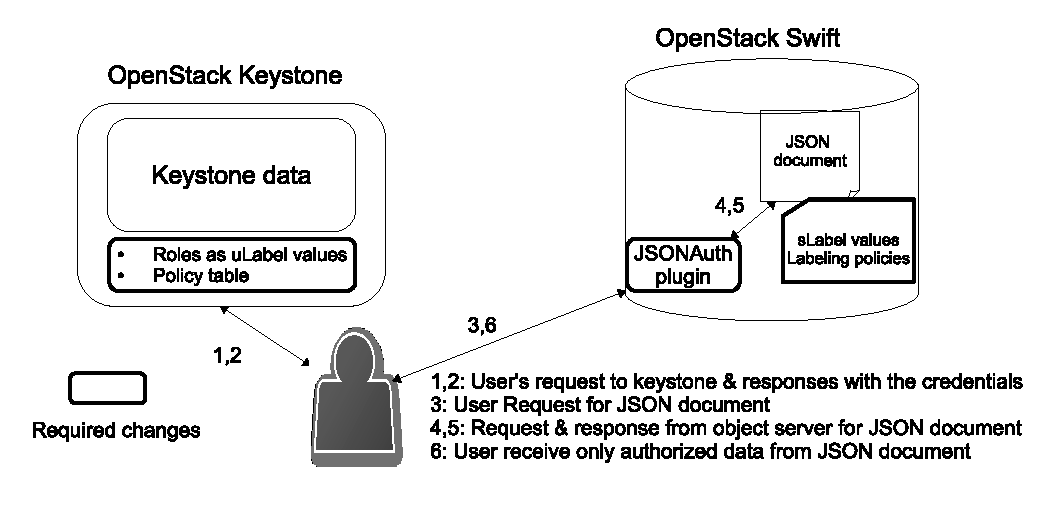
\includegraphics[width=.9\textwidth]{NSS16/implementation-in-swift}
 		\caption{Implementation in OpenStack IaaS cloud platform}
 		\label{fig:implementation-in-swift}
 	\end{figure}
 

We have implemented our proposed operational model and path-based labeling scheme in OpenStack IaaS cloud platform using OpenStack Keystone as the authorization service provider and OpenStack Swift as the storage service provider. Our choice of OpenStack is motivated by its support for independent and inter-operable  services and a well defined RESTful API set.

We have modified OpenStack Keystone and Swift services to accommodate required changes. A reference architecture of our testbed is given in Figure \ref{fig:reference-implementation-architecture}. Details of the implementation is shown in Figure \ref{fig:implementation-in-swift-a}. Required changes are presented as highlighted rectangles in Figure \ref{fig:implementation-in-swift-a}.

\subsection{Changes in OpenStack Keystone}

 OpenStack Keystone uses roles and role-based policies to provide authorization decisions. In our implementation, we uses roles to hold user-label attribute values. A set of valid security-label values are also stored as part of the Keystone service.
 
 Among two different types of policies, authorization and labeling policies, the former is managed in the Keystone service. We assume, a higher level administrators (possibly at the level of organization) adds, removes or updates these authorization policies. We add a policy table in Keystone database to store these enumerated authorization policies. 

\subsection{Changes in OpenStack Swift}

In Swift side, we store \textit{security-label} values assigned to JSON objects and path-based labeling policies applied to them.  Security-label values and labeling policies are stored as metadata of the stored objects, which are JSON documents in this case. For simplicity, we assume object owner (Swift account holder in this case) can update security-label values or labeling policies for a stored JSON document. 


 During the evaluation, we intercept every request to Swift (from the Swift-proxy server) and reroute the request to be passed through \textit{JSONAuth plugin}, if it is a request for a JSON document. In this case, the request additionally carries a requested path and authorization policies applicable to the user. JSONAuth plug-in retrieves the requested JSON document, applies path-based labeling policies to annotate the document and uses authorization policies to determine if the user is authorized for the requested content of the file. 

\subsection{Evaluation}

 \begin{figure} [t]
 	\centering
 	\includegraphics[width=.9\textwidth]{NSS16/performance}
 	\caption{Performance evaluation}
 	\label{fig:performance-a}
 \end{figure}


An evaluation of our implementation is shown in Figure \ref{fig:performance-a}. The evaluation has been made against concurrent download requests to the Swift proxy server. The X-axis shows size of the JSON document requested for download while the Y-axis shows the average download time for 10 concurrent request. Our evaluation shows a performance hit of nearly 60\% over no authorization protection.
%\textbf{Performance}



	
%\section{Content-Level Protection for OpenStack Swift}

%	In this section, we show how we have extended our enforcement of \eapABAC{} specified in the last section to enable content-level protection for objects stored in OpenStack Swift.

%	\subsection{Motivation}
%	Swift, the object storage service from OpenStack cloud computing platform is used for storing, managing and retrieving large amounts of data. Inside Swift, uploaded files, also known as objects, are organized in containers. Objects inside a container are managed to be accessible or restricted from users through  Access Control Lists (ACLs). Swift ACL, at the finest level, works on a Swift object  enforcing who can or cannot access the object. Once an object is accessible to some one, he gets the full content of the object. Thus Swift ACL is an ``all or nothing'' approach.

%	In this work, we allow Swift users to specify access control at the content level of a Swift object. The content level policy describes who can access which part of a Swift object. When a request comes for downloading (i.e. read) an object, we check content level policy along with the ACL for the object. The response of the request is a partial content of the requested object based on the credential of the requester. Our prototype implementation is done on Swift objects of content type ``application/json''.
	
%	%\subsection{Motivation}
OpenStack  Swift is a highly deployed open source cloud storage solution. With its unlimited storage capacity, it is used to store any number of large or small objects. In Swift terminology, uploaded documents are called objects.  A user can  upload or download an object using well defined APIs or available Swift client programs. But not everyone can download (i.e. read) every object stored in Swift. In order to maintain who can or cannot access an object, Swift uses Access Control Lists (ACLs). ACL specifies who can or cannot access an object. Unfortunately, the ACL based approach for Swift is an `all or nothing' approach in a way that an user can either download (i.e. read) the whole object or cannot download it at all.

We propose a content level access control mechanism for objects  stored in Swift.  This approach lets Swift users specify who can access which part of a Swift object. To give a concrete example, consider that a hospital stores its patient records  as  Swift objects. These records should be accessed differently by different personnel. For example, `doctors' can see certain part  while the `billing accountant' can see other part of the record. Our implementation would let the data publisher specify policies expressing who can see which part of the data.

Our prototype implementation is based on JSON formatted documents. We use JSON data because recently JSON has gained immense commercial popularity which is reflected by developments including JSON document database such as MongoDB supported by the OpenStack cloud platform, Twitter's latest API (v 1.1) which supports only JSON data and so on.

%\subsection{OpenStack background}

\subsubsection{Swift}

Swift is a highly available, distributed, eventually consistent object storage which can operate standalone or integrated with the rest of the OpenStack cloud computing platform. It is used  to store lots of data efficiently, safely, and cheaply using a scalable redundant storage system \cite{swift-definition}. As opposed to conventional storage architectures like file systems which manage data using file hierarchy and block storage, Swift manages data as objects. Each object typically includes the data itself, a variable amount of metadata, and a globally unique identifier.

%\textbf{Swift Servers}: 
Using its well defined RESTful API \cite{swift-api}, users can upload or download objects to and from Swift storage. Inside Swift, objects are organized into containers which is similar to directories in a filesystem except that Swift containers cannot be nested. Again, a user is associated with a Swift account and can have multiple containers associated with the account. In order to manage user accounts, user containers and objects inside a container, Swift uses an Account Server, a Container Server and Object Servers correspondingly.

When a user corresponding to a user account requests for an object inside a container (either for uploading or downloading), the Account Server looks for the account first in its account database and finds associated containers with the account. The Container Server then checks the container database to find whether the requested object exists in the specified container and finally the Object Server looks into `object databases' to find retrieval information about the object. In order to retrieve an object, the Proxy Server needs to know which of the Object Servers are storing the object, and path of the object in the local filesystem of that server.



% For interacting with objects stored inside Swift storage, it provides a RESTful API using HTTP request methods (e.g. GET, PUT, DELETE etc).


\subsubsection{Swift ACL}
	Once an object is stored in Swift, who can or cannot access the object is determined by Swift Access Control List (ACL).  Swift has  different levels of ACL---Account level ACL, and Container level ACL, for example. Container level ACL is associated with containers in term of a \emph{read} action, or \emph{write} action  or \emph{listing} action. If a user is authorized read action on a container through read ACL, he or she can read or download objects from the container. Similarly, write ACL enables uploading an object into a container and listing ACL enables the list operation on the container. Account ACLs, on the other hand, allow users to grant account-level access to other users.  Of these two types of ACL, Container level ACL is  finer grained in that different containers of a single account can be configured differently. Nonetheless, Swift ACL is limited in the following ways.
	
\begin{itemize}
	\item  Once an object is set accessible  to someone, he or she gets the full content of the object. But  there can be some sensitive information that the publisher wants to hide out.
		
	 \item  Swift ACL allows  sharing an object with others, but it does not allow to share objects selectively at the content level.
	
\end{itemize}	
%--------------Following section is commented---------------------
%Account level ACL is specified in terms  of  \emph{read-only}, \emph{read-write} and \emph{admin} operation. For example, anyone having \emph{read-only} ACL on the account level can do a listing on all the containers or read all objects of all containers associated with the Account.
%Using ACL, it is possible to specify who can access objects inside the container. Examples of some supported ACLs are `read' ACL, `write' ACL, `listing' ACL and so on. With Swift ACL, we can either specify a positive list and a negative list. For example, a read acl with following ACL value \emph{ `.referrer:*'} allows everyone to read or download objects from corresponding container.  On the other hand, value of \emph{`.referrer:*-example.com} as read ACL, remove read permission for request coming from example.com as a referrer.

%A point to note is that Swift ACL either allows and denies access to an object. Once  ACL allows access to an object, the requester gets full content of the object. So, essentially, ACL based access is an `all or nothing' approach and cannot be used to share a Swift object selectively among different users.

%--------------commenting ends here---------------------


%\subsection{JSON (JavaScript Object Notation)}

%JSON or JavaScript Object Notation is a data representation format which uses human readable text to represent data. In JSON, data is represented in one of two forms---as an \emph{object} or as an \emph{array of values}. A JSON object is defined as a collection of \emph {key-value} or \emph {attribute-value} pairs where a \emph {key} or an \emph {attribute}\footnote{To avoid confusion with the use of \emph{attribute} for attribute-based access control we will exclusively use the term \emph{key} in this paper.} is simply a string representing a name  and a \emph {value} which is either one of the following primitive types---string, number, boolean (true or false), null or another object or an array. On the other hand, an array is defined as a set of an ordered collection of \emph {values} (as defined above) starting from index zero. The formal definition of JSON data format is given in   \cite{json-official-website}. JSON structure has following characteristics

%\begin{enumerate}
%  \item A JSON document forms a hierarchical structure which is a rooted tree.
%  \item In the rooted tree, leaf nodes represent text data of the document and non-leaf nodes are used to give the data a name and thus  organize it.
%  \item In the rooted tree, a node can be uniquely identified by traversing the document from the root node to the target node.
%\end{enumerate}



%JSON or JavaScript Object Notation is a data representation format which uses human readable text to represent data. In JSON, data is represented in one of two forms -  as an object or as an array of values. In our implementation, we use a JSON object or a JSON array as the minimum protection unit and assign object-label values on them. Figure \ref{fig:labelled-json-data} shows a sample JSON document with its objects being labelled as `personal', `public', `protected' and so on. In simple situations, roles of a user can be used as his user-label values. A simple policy for the given JSON data is \emph{ (`personal', read, `patient')} which means that JSON objects labelled with `personal' can only be read by users having a label of `patient'.


\begin{figure}
  \centering
    
\includegraphics[width=0.3\textwidth]{CODASPY15/json-data}
 \caption{A sample JSON Document containing   records of an employee.}
   \label{fig:json-data}
\end{figure}



\subsection{Label Based Access Control}
In order to protect a JSON document stored as a Swift object, we assign each JSON item (i.e. value of a JSON key) an \emph{object-label} and each user a \emph{user-label}. Then we specify policies  in the form of  (\emph{user-label} values, \emph{action},  \emph{object-label} values)   which means that objects labeled with any of `object-label' values are allowed to be accessed by the users labeled with any of  `user-label' values for the specific `action'. Here we present an informal description of the model and its open source implementation is available in \cite{labac}.

\begin{figure*}
\centering
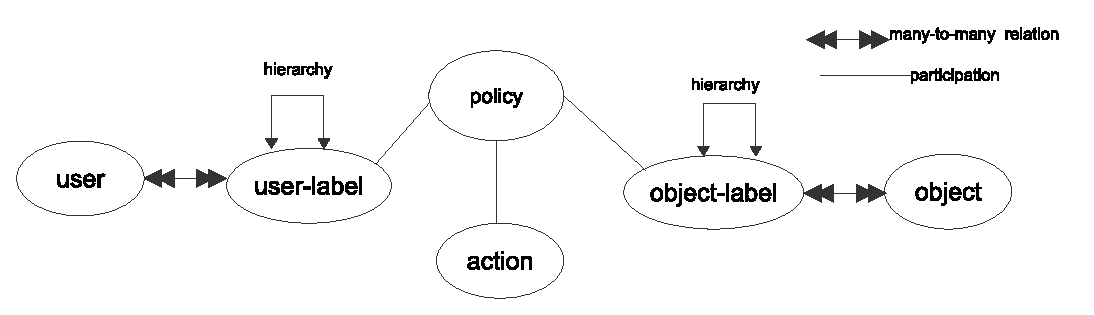
\epsfig{file=CODASPY15/labac-model.eps}
\caption{Label Based Access Control Model.}
\label{fig:labac-model}
\end{figure*}


\subsubsection{Model Components}

In LaBAC (Figure \ref{fig:labac-model}), we have one attribute assigned to objects and one attribute assigned to users. Object attribute is named  \emph{object-label} and user attribute is named \emph{user-label}. These attributes are set valued attributes and the values of the attributes may form a partial order.
%Note that, both object-label and user-label are a special type of attribute  which we do not elaborate here for brevity.

\emph{Object}: Object is any resource we want to protect with the model. Examples include a JSON document or items inside a JSON document. 

\emph{Object-label}: Object-label is the attribute assigned on the objects. The values of this attribute  may form a partial order.

\emph{User} and \emph{user-label}: User-label is the attribute assigned on each user. In a simple case, user-label values can be the set of roles assigned to the user. The values of this attribute may form a partial order.

\emph{Action}: Action is the list of available actions to be exercised on the objects. 
%Although, it is possible to have hierarchy on action, to keep the model simple we do not introduce action hierarchy.

\emph{Policy}: A policy in this model is a tuple of (\emph{user-label} values, \emph{action},  \emph{object-label} values). The policy is interpreted such that objects labeled with any of `object-label' values are allowed to be accessed by the users labeled with any of  `user-label' values for the specific `action'.

\emph{Attribute Hierarchy}: In our model, both object-label and user-label values  may form a hierarchy or more specifically a partial order. The effect of attribute hierarchy is shown in Figure \ref{fig:attribute-hierarchy}. As we can see in the figure, if a policy allows an action for user-label $l_{uj}$ on object-label $l_{oj}$, due to the attribute hierarchy, all users having a equivalent or senior label than $l_{uj}$ can also access object-label $l_{oj}$ or its junior labels.

\begin{figure}
  \centering
    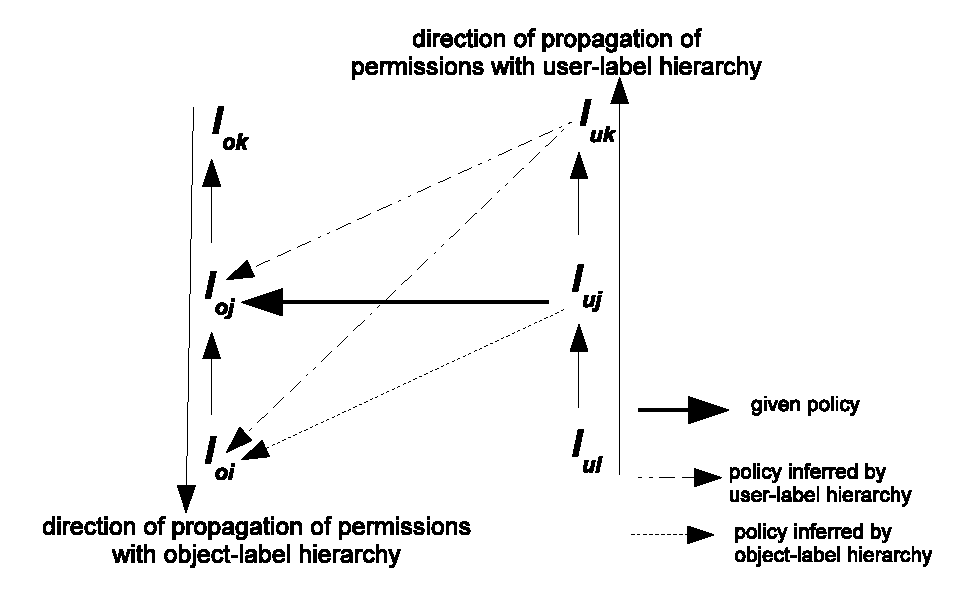
\includegraphics[width=0.5\textwidth]{CODASPY15/attribute-hierarchy}
 \caption{Propagation of permission with attribute hierarchy.}
 \label{fig:attribute-hierarchy}
\end{figure}

 \subsection{Content Level Protection}


Swift ACL specifies who can or cannot access a Swift object but it cannot   specify who can access which part of the object.  In order to specify security policies at the content level, Swift has to be aware of the content type and data format of the object. In our case, we addressed Swift objects of content-type \emph{`application/json'} which is  standard JSON format. How our protection mechanism works  is summarized below.

\begin{itemize}
\item JSON items to be protected are identified using JSONPath. For example, SSN in JSON data given in Fig. \ref{fig:json-data} is identified using JSONPath `\$.personal\_record.ide ntification.SSN'.
\item  \emph{object-label} values are assigned on the specified JSON item. For example, to specify that SSN is a sensitive information, we assign a label \emph{`sensitive'} on JSONPath `\$.personal\_record.identification.SSN'.

\item We use LaBAC policy to specify who can access (read) which \emph{object-label}. For example, if only users with user-label `manager' can access \emph{sensitive} information, then we specify the LaBAC policy \emph{(`manager', read, `sensitive')}.

\end{itemize}

When using JSONPath to identify a JSON item, one may want to  specify value at the path  as a condition. For example, salary information (given in Fig. \ref{fig:json-data}) is sensitive only if the salary is greater than 50,000. Furthermore, it is also possible to protect one item based on value of a different item. For example, identification information (specified by JSONPath   `\$.personal\_record.identification') of a user is sensitive when his salary is greater than 50,000.

\subsection{Labeling  JSON Items}
If the JSON document is large, labeling all JSON items can be tedious. In order to reduce labeling effort, we propagate label assigned on a JSON item to all its descendant items. For example, if the \emph{personal\_record}  item (Fig. \ref{fig:json-data}) is labeled \emph{sensitive}, then all its descendant nodes (name, DOB, identification, DL, SSN) are also labeled  \emph{sensitive}.




\input{CODASPY15/content-level-protection.tex}

\subsection{Implementation}
%In our implementation, we are interesting in the following use case.

% \emph{Alice has an account with OpenStack Swift. She has an object `data.json' in a Swift container. She likes to share this object with her colleagues Bob and Charlie so that they can only see selective content of 'data.json' that she has authorized  them.}

%In the rest of this section, we specify required changes in Swift.




\subsubsection{Changes in Swift Object Server}

 We have extended  the logic of Swift Object Server. In the existing implementation, when a request comes for downloading of an object, Object Server checks the ACL and if the object is allowed by ACL, the Object Server reads the object from the disk and pass the whole content to the requester through Proxy-server.

\begin{figure}
  \centering
    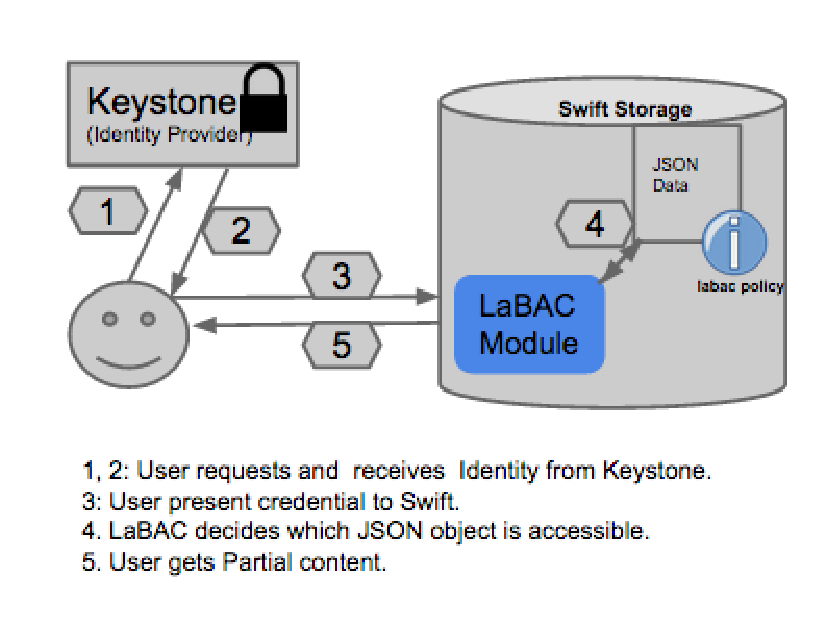
\includegraphics[width=0.5\textwidth]{CODASPY15/labac-implementation.eps}
 \caption{ Required Changes in Swift Object Server for Our Extension}
   \label{fig:implementation-in-swift}
\end{figure}
	
	In our implementation (see Figure \ref{fig:implementation-in-swift}), if the ACL denies the request, no further check is made and user gets corresponding error messages. Otherwise,  we retrieve the object, content level policy (stored with the Swift Object as metadata), user credential (user-label specifically which is the roles of the user maintained by Keystone) and pass them to the LaBAC module. LaBAC module processes the requested object based on the policy and user credential, and removes unauthorized content from the object. Then only the authorized partial content of the object is returned to the requester through Swift Proxy-server.
	
Note that in the implementation,  we have used OpenStack Keystone \cite{keystone} as the identity provider and we have mapped user roles provided by the Keystone as user-label values of the requester.

\subsubsection{Storing of Policies}
	In our implementation, we have two different types of policies---LaBAC policies in the form of (\emph{user-label} values, \emph{action},  \emph{object-label} values) and content-level policies in the form of \emph{(JSONPath, \{Labels\})}. All of these policies are stored as the metadata of the Swift object. Note that the Swift object is the JSON document itself.
	
	One challenge of storing policies as metadata of Swift object is that Swift does not allow a single metadata item larger than 256 bytes. To circumvent this limitation, policies are stored as multiple metadata items.


%\subsection{Changes in Request Header}

%In order to associate LaBAC and content-label policy with the Swift object, we need to add a new request header namely, \textbf{--cbac-policy}. The values of --cbac-policy header is the policies required for our protection model.

\subsection{ Limitation of the Implementation}

	 Our prototype implementation works only on objects of type `application/json'. If requested object is not a JSON file or the requested object does not have content level policy set, the requester gets full content of the file.
	

\subsection{Performance}
In order to analyze the performance of our implementation, we compared the download time of a Swift object enabling content policy and without enabling content policy. Our analysis (Figure \ref{fig:performance})  shows that our implementation works well for Swift object of size smaller than 100KB beyond which CLAC does not work efficiently.  We believe this is because our implementation exhausts memory very soon. We conjecture that  pre-labeling objects and enforcing access control in divide-and-concur fashion may improve performance.
\begin{figure}
  \centering
    \includegraphics[width=0.5\textwidth]{CODASPY15/performance.eps}
 \caption{ Performance of our Implementation}
   \label{fig:performance}
\end{figure}

%\section{Related Work}
%There have  been very few works for access control of JSON data, although JSON and XML data are very similar and lots of works has been done at the content level for XML data \cite{ bertino2000specifying,damiani2002fine}.  Additionally there are prior works that apply object labels at the content level \cite{adam2002content} for access control purposes. But, to the best of our knowledge, applying content level access control for the application context of OpenStack Swift has not yet been  performed. 